% XeLaTeX can use any Mac OS X font. See the setromanfont command below.
% Input to XeLaTeX is full Unicode, so Unicode characters can be typed directly into the source.

% The next lines tell TeXShop to typeset with xelatex, and to open and save the source with Unicode encoding.

%!TEX TS-program = xelatex
%!TEX encoding = UTF-8 Unicode

\documentclass[12pt]{article}
\usepackage{geometry}                % See geometry.pdf to learn the layout options. There are lots.
\geometry{letterpaper}                   % ... or a4paper or a5paper or ... 

\geometry{left=1in}
\geometry{right=1in}
\geometry{bottom=1.9in}
\geometry{top=1in}

%
%Setting the font
%
\usepackage{times}

%
%Rotating tables (e.g. sideways when too long)
%
\usepackage{rotating}

%
%For multiple rows in tables
%
\usepackage{multirow}

% 
%Line numbering in verse environment
%
\usepackage{lineno} 

%
%Fancy-header package to modify header/page numbering (insert last name)
%
\usepackage{fancyhdr}
\pagestyle{fancy}
\lhead{} 
\chead{} 
\rhead{Quan \thepage} 
\lfoot{} 
\cfoot{} 
\rfoot{} 
\renewcommand{\headrulewidth}{0pt} 
\renewcommand{\footrulewidth}{0pt} 
%To make sure we actually have header 0.5in away from top edge
%12pt is one-sixth of an inch. Subtract this from 0.5in to get headsep value
\setlength{\headsep}{1in}

\usepackage{setspace}
\doublespacing

\usepackage{apacite}
\usepackage{url}

% used to count words
\usepackage{xesearch}
\newcounter{words}
\newenvironment{wordcount}{%
  \setcounter{words}{0}
  \SearchList!{wordcount}{\stepcounter{words}}
    {a?,b?,c?,d?,e?,f?,g?,h?,i?,j?,k?,l?,m?,
    n?,o?,p?,q?,r?,s?,t?,u?,v?,w?,x?,y?,z?,
    1?,2?,3?,4?,5?,6?,7?,8?,9?,0?}
  \UndoBoundary{'}
  \SearchOrder{p;}}{%
  \StopSearching}


\title{}
\author{}
\date{}                                           % Activate to display a given date or no date

\begin{document}

\begin{flushleft}
%%%%First page name, class, etc
Shengjie Quan\\
Professor: Praveen Kumar\\
CSE 5234 \\
\today \\

%%%%Title
\begin{center}
\textbf
CSE 5234 Paper
\end{center}

%%%%Changes paragraph indentation to 0.5in
\setlength{\parindent}{0.5in}
In an enterprise, a main challenge arises these days is that having possession of massive amount of data accumulated during business, seldom can the enterprise utilize them to extract useful information from the data. The major obstacle besides the massive quantity being challenge to manipulating on the data is that data most likely in numerical form is good for computer to process but bad for human to interpret. Data visualization is thus introduce into enterprise computing to solve this problem. Data visualization is in fact a data mining strategy in the sense of extracting useful information from data while abstracting ``in some schematic form, including attributes or variables for the units of information'' thus providing result that can be easily interpreted by human \cite{mith}. Data visualization intuitively belongs to data domain of enterprise computing; however, it is not being isolated in data domain. The result produced can have great impact on the business operation of an enterprise. Thus data visualization is more and more engaged in reporting and business intelligence.

The most current data visualization technology is quantitative messages which includes the communication of the following messages\cite{emmm}:
\begin{singlespace}
\begin{itemize}
	\item Time-series
	\item Ranking
	\item Part-to-whole
	\item Deviation
	\item Frequency distribution
	\item Correlation
	\item Nominal comparison
	\item Geographic or geospatial
\end{itemize}
\end{singlespace}
Despite the complex definition or the concept of any of the terms above, one fact falls into our observation is that all of them are statistics. Data visualization currently is implemented by statistic plots such as bar chat, scatter plot, etc which carries statistic information above. This implementation approach is quite nature due to the fact that statistics summarize the data which reduce the quantity and statistic plots are traditional way to present the statistics summary of the data. A usable implementation however is typically far more complex than just displaying a bar chat (or just a statistic plot). The complexity is laid on the fact that without choosing the correct parameters (e.g. range, etc) to display a plot, the information and pattern associated with the information may not be revealed. Even choosing the type of the plot may also impact the presentation of the information with in the data. Also automate the process of choosing a proper plot type and plot with proper parameter is of great complexity.

In terms of available commercial off-the-shelf (COTS) software, below is a list:
\begin{singlespace}
\begin{itemize}
	\item Sisense
	\item Zoho Reports
	\item Dundas Bi
	\item Idashboards
	\item Salesforce Analytics Cloud
	\item Domo
	\item Chartio
	\item Gooddata
\end{itemize}
\end{singlespace}
Since the current approach of data visualization being statistics, any statistic tools such as \emph{R} can also be used as a data visualization software. One newly released software of particular interests is Amazon AWS Quicksight. Figure 1 is a screenshot of the software.
\begin{figure}[h]
\centering
        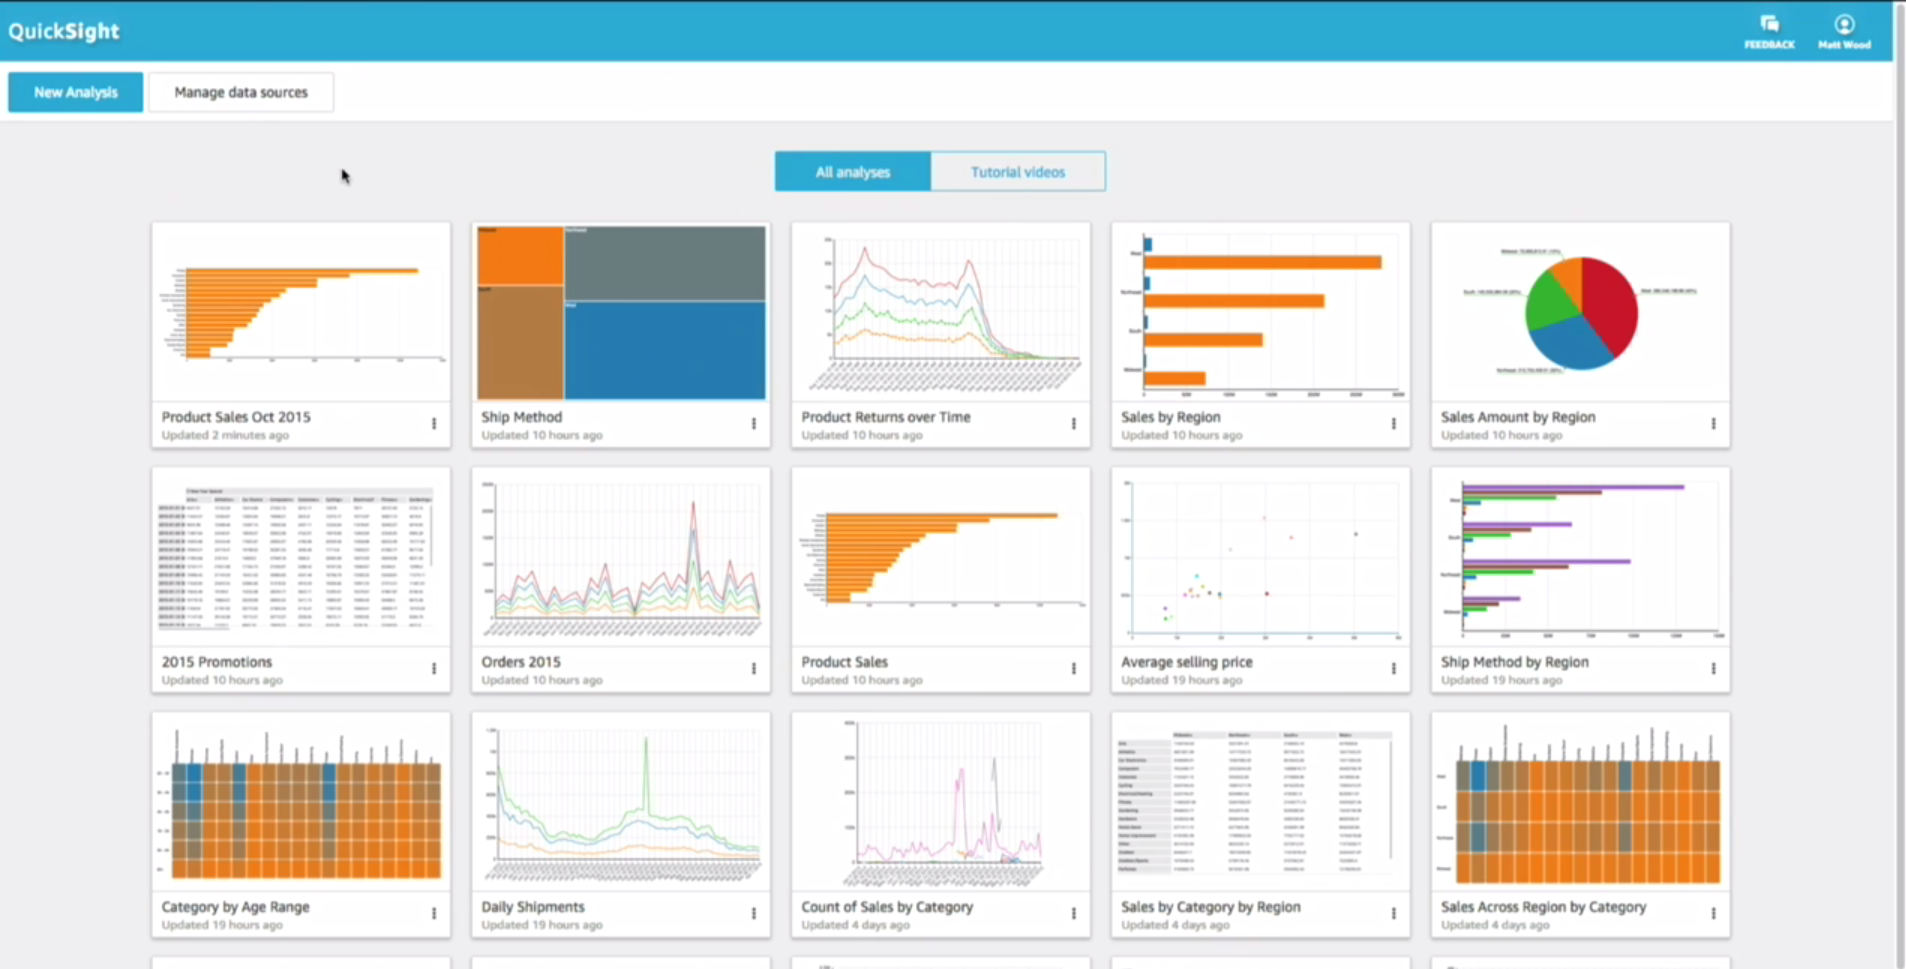
\includegraphics[totalheight=9cm]{screenshot.png}
    \caption{Amazon AWS Quicksight Screenshot}
\end{figure}
The reason AWS Quicksight being competitive among software of similar functionality is not only because of its deep integration with already exist database software which company may store massive data in, but also because of the fact that AWS Quicksight has ``built-in suggestion engine that provides you with recommended visualizations based on the properties of the underlying datasets'' \cite{awsq}. As I mentioned previously, automating the process of choosing a proper plot type and plot with proper parameter is of great complexity. Moreover, such process is valuable because it fact out the bias when performing the process by a person. Thus AWS Quicksight should in theory produce more objective result.

To sum up, data visualization is an attempt by enterprise to mine information from data and present the information in a meaningful way. It is a data domain problem that falls in reporting and business intelligence category. Data visualization is challenging because both the fact that calculation involves massive data and the fact that produce proper presentation of data efficiently is complex. Data visualization is heavily relied on statistics and converge with statistics in many areas. COTS software is widely available and statistics softwares are acceptable alternatives with AWS Quicksight being quite competitive in this field.
\end{flushleft}
\clearpage

\begin{center}
\bibliographystyle{apacite}
\bibliography{bib}
\end{center}
\end{document}  